%allgemeine Formatangaben
\documentclass[
 a4paper,                       % Papierformat
 12pt,                          % Schriftgr\"o\ss{}e
 ngerman,                       % f\"ur Umlaute, Silbentrennung etc.
 titlepage,                     % es wird eine Titelseite verwendet
 bibliography=totoc,                    % Literaturverzeichnis im Inhaltsverzeichnis auff\"uhren
 listof=totoc,                      % Verzeichnisse im Inhaltsverzeichnis auff\"uhren
 twoside,                       % einseitiges Dokument
 openright,
 captions=nooneline,                    % einzeilige Gleitobjekttitel ohne Sonderbehandlung wie mehrzeilige Gleitobjekttitel behandeln
 numbers=noenddot,                  % \"Uberschriften-??Nummerierung ohne Punkt am Ende
 parskip=half,                      % zwischen Abs\"atzen wird eine halbe Zeile eingef\"ugt
 ]{scrbook} %scrartcl



%http://tex.stackexchange.com/questions/21904/input-and-absolute-paths
\makeatletter
\def\input@path{{./content/resources/}} % {../r/doc/}
\makeatother

% \graphicspath{{./content/resources/}}

% Anpassung an Landessprache
\usepackage[ngerman]{babel}
 
% Verwenden von Sonderzeichen und Silbentrennung
\usepackage[utf8]{inputenc}
\usepackage[T1]{fontenc}
% \DeclareUnicodeCharacter{0008}{}
% \DeclareUnicodeCharacter{00A0}{~}
\usepackage{textcomp} 					% Euro-Zeichen und andere
\usepackage[babel,german=quotes]{csquotes}		% Anf\"uhrungszeichen
\RequirePackage[ngerman=ngerman-x-latest]{hyphsubst} 	% erweiterte Silbentrennung

\usepackage{multicol}                   %

% Befehle aus AMSTeX f\"ur mathematische Symbole z.B. \boldsymbol \mathbb
\usepackage{amsmath,amsfonts,amssymb,amsthm}

% Zeilenabst\"ande und Seitenr\"ander 
\usepackage{setspace}
\usepackage[left=3cm,right=3cm]{geometry}

% Einbinden von JPG-Grafiken
\usepackage{graphicx}

% zum Umflie\ss{}en von Bildern
% Verwendung unter http://de.wikibooks.org/wiki/LaTeX-Kompendium:_Baukastensystem#textumflossene_Bilder
\usepackage{floatflt}

% Eigene Flie\ss{}umgebungen erzeugen
\usepackage{float}


% Verwendung von vordefinierten Farbnamen zur Colorierung
% Palette und Verwendung unter http://kitt.cl.uzh.ch/kitt/CLinZ.CH/src/Kurse/archiv/LaTeX-Kurs-Farben.pdf
\usepackage{xcolor} 

% Tabellen
\usepackage{array}
\usepackage{longtable}
\usepackage{multirow}
\usepackage[normalem]{ulem}                   %

% einfache Grafiken im Code
% Einf\"uhrung unter http://www.math.uni-rostock.de/~dittmer/bsp/pstricks-bsp.pdf
\usepackage{pstricks}

\usepackage{pst-plot}					% Darstellung von Graphen
\usepackage{pstricks-add}				%
\usepackage{pst-tree}					% Darstellung von B\"aumen

%--- Definitionen mit Schattierung
\usepackage{shadethm}                   %

% Quellcodeansichten
\usepackage{verbatim}
\usepackage{moreverb} 					% f\"ur erweiterte Optionen der verbatim Umgebung
% Befehle und Beispiele unter http://www.ctex.org/documents/packages/verbatim/moreverb.pdf
\usepackage{listings} 					% f\"ur angepasste Quellcodeansichten siehe
% Kurzeinf\"uhrung unter http://blog.robert-kummer.de/2006/04/latex-quellcode-listing.html

% Glossar und Abbildungsverzeichnis
\usepackage[
nonumberlist, 						%keine Seitenzahlen anzeigen
acronym,      						%ein Abk\"urzungsverzeichnis erstellen
toc          						%Eintr\"age im Inhaltsverzeichnis
]      							%im Inhaltsverzeichnis auf section-Ebene erscheinen
{glossaries}



% Stichwortverzeichnis
\usepackage{makeidx}					% Erzeugung eines Stichwortverzeichnisses

% verlinktes und Farblich angepasstes Inhaltsverzeichnis
\usepackage[colorlinks=true,
linkcolor=InterneLinkfarbe,
urlcolor=ExterneLinkfarbe]{hyperref}
\usepackage[all]{hypcap}

% URL verlinken, lange URLs umbrechen
\usepackage{url}

% sorgt daf\"ur, dass Leerzeichen hinter parameterlosen Makros nicht als Makroendezeichen interpretiert werden
\usepackage{xspace}

% Beschriftungen f\"ur Abbildungen und Tabellen
\usepackage{caption}
\usepackage{subcaption}

% Entwicklerwarnmeldungen entfernen
\usepackage{scrhack}

\usepackage{algorithm}
\usepackage{algpseudocode}

\usepackage{calc}


\usepackage{hyperref}
%\usepackage{hdvips}					% soll das Problem verhindern, dass Akronyme nicht umgebrochen werden

\usepackage{fancyvrb}
\usepackage{fancyhdr}

\usepackage[backend=biber,natbib=true,style=ieee,dashed=false,date=long,url=false,doi=false,isbn=false]{biblatex}
% \bibliography{content/headfoot/library,content/headfoot/mylibrary}
\addbibresource{content/headfoot/library.bib}
\addbibresource{content/headfoot/mylibrary.bib}
% \bibliographystyle{plain}

\usepackage{blindtext}

% for using R Sweave
\usepackage{Sweave}
					% einbinden der verwendeten Latex-Pakete

\newcommand{\thesistitle}{Title}
\newcommand{\thesissubtitle}{Untertitel}
\newcommand{\thesis}{Masterarbeit}
\newcommand{\university}{Universität Leipzig}
\newcommand{\department}{Institut für Informatik}
\newcommand{\universityshort}{Uni Leipzig}
\newcommand{\departmentshort}{IfI}
\newcommand{\thesisauthor}{Name}
\newcommand{\course}{Informatik Master}
\newcommand{\slidessubject}{Schwarmintelligenz und Komplexe Systeme}
\newcommand{\matrikelnr}{0000000}
\newcommand{\place}{Leipzig}


% Deckblatt
\newcommand{\abschlussart}{Master of Science (M.Sc.)}
\newcommand{\erstgutachter}{Prof. Dr. X}
\newcommand{\zweitgutachter}{Some Other}
 				% einbinden von pers\"onlichen Daten

\newcommand{\leadingzero}[1]{\ifnum #1<10 0\the#1\else\the#1\fi} 	% fügt bei einstelligen Zahlen eine f\"uhrende 0 ein
\newcommand{\Ind}[1]{#1\index{#1}}					% Eintrag ins Stichwortverzeichnis mit direkter Ausgabe
\newcommand{\getLable}[1]{\ref{#1} auf Seite \pageref{#1}}		% erm\"oglicht folgende Ausgabe "Kapitel 1.2 auf Seite 7"

					% Erg\"anzende Befehle

% \floatstyle{ruled}
\newfloat{program}{bhp}{lop}
\floatname{program}{Pseudocode}

\onehalfspacing 					% 1,5facher Zeilenabstand

%\geometry{left=2.5cm,right=2.5cm,top=1.5cm,bottom=1cm,includeheadfoot}

% \definecolor{InterneLinkfarbe}{rgb}{0.1,0.1,0.3}    % Farbliche Absetzung von externen Links
\definecolor{InterneLinkfarbe}{rgb}{0.0,0.0,0.0} 	% Farbliche Absetzung von externen Links
\definecolor{ExterneLinkfarbe}{rgb}{0.1,0.1,0.7}	% Farbliche Absetzung von internen Links
\definecolor{dunkelgrau}{rgb}{0.8,0.8,0.8}      %
\definecolor{hellgrau}{rgb}{0.95,0.95,0.95}     %
\definecolor{orange}{rgb}{1,0.7,0}          %
\definecolor{darkgreen}{rgb}{0,0.5,0}           %
\definecolor{lila}{rgb}{0.5,0,0.5}          %

% Einstellungen f\"ur Fu\ss{}noten:
\captionsetup{font=footnotesize,labelfont=sc,singlelinecheck=true,margin={5mm,5mm}}

% Stil der Quellenangabe
% \bibliographystyle{ieeetr} % apalike,alphadin,ieeetr,authordate,harvard

\theoremstyle{definition}
\newtheorem{exmp}{Beispiel}

%Ausschluss von Schusterjungen
\clubpenalty = 10000
%Ausschluss von Hurenkindern
\widowpenalty = 10000
\displaywidowpenalty=10000

% Befehle, die Umlaute ausgeben, f\"uhren zu Fehlern, wenn sie hyperref als Optionen \"ubergeben werden
\hypersetup{
    pdftitle={\thesistitle \thesissubtitle},
    pdfauthor={\thesisauthor},
    pdfcreator={\thesisauthor},
    pdfsubject={\thesistitle \thesissubtitle},
    pdfkeywords={\thesistitle \thesissubtitle},
    citecolor=black
}

% Beispiel f\"ur eine Listings-Codeumbebungen
% Bei mehreren Definitionen empfielt sich das auslagern in eine externe Datei

%TODO: MATLAB einf\"ugen
\lstloadlanguages{Python} %Java
% \lstset{
% 	frame=tb,
% 	framesep=5pt,
% 	basicstyle=\footnotesize\ttfamily,
% 	showstringspaces=false,
% 	keywordstyle=\ttfamily\bfseries\color{CadetBlue},
% 	identifierstyle=\ttfamily,
% 	stringstyle=\ttfamily\color{OliveGreen},
% 	commentstyle=\color{GrayBlue},
% 	rulecolor=\color{Gray},
% 	xleftmargin=5pt,
% 	xrightmargin=5pt,
% 	aboveskip=\bigskipamount,
% 	belowskip=\bigskipamount
% }

%Den Punkt am Ende jeder Beschreibung deaktivieren
\renewcommand*{\glspostdescription}{}

%Silbentrennung

\hyphenchar\font=\string"7F
\hyphenation{Wahr-schein-lich-keit}


%Glossar-Befehle anschalten
\newglossary[slg]{symbolslist}{syi}{syg}{Symbolverzeichnis}
\newglossarystyle{customlong}{
    \setglossarystyle{long}
    % I use this to prevent a different vertical spacing from x2 to y than from x1 to x2
    \renewcommand{\glsgroupskip}{}
}
\makeglossaries
\glsenablehyper
%Befehle f\"ur Abk\"urzungen
%Eine Abk\"urzung mit Glossareintrag

\newacronym{acro:API}{API}{Programmierschnittstelle\protect\glsadd{glos:API}}
\newacronym{acro:GUI}{GUI}{Grafische Benutzeroberfläche\protect\glsadd{glos:GUI}}

%\newacronym{acro:}{}{\protect\glsadd{}}
%\newacronym{acro:}{}{}

\newglossaryentry{glos:AD}{
    name={Active Directory},
    description={a komplex thing},
    plural=more things
    }

\newglossaryentry{glos:API}{
    type=\acronymtype,
    name={API},
    description={Programmierschnittstelle},
    first={Programmierschnittstelle (API)\glsadd{glos:APIG}},
    see=[Glossary:]{glos:APIG}
    }

\newglossaryentry{glos:GUI}{
    name={Grafische Benutzeroberfläche (engl. graphical user interface)},
    description={Bietet dem Benutzer eines Programms die Möglichkeit, es mittels graphischen Symbolen und Steuerelementen zu bedienen.},
    plural=more things
    }

\newcommand{\sign}{\mathop{\mathrm{sgn}}\nolimits}
\newcommand{\err}{\mathop{\mathrm{err}}\nolimits} % \nolimits
\newcommand{\card}{\mathop{\mathrm{card}}\nolimits} % \nolimits

% \newglossaryentry{symb:}{
% name=$$,
% description={},
% sort=,
% type=symbolslist
% }


\newglossaryentry{symb:Lambda}{
name=$\lambda$,
description={Eine beliebige Zahl, mit der der nachfolgende Ausdruck
multipliziert wird},
sort=symbollambda, type=symbolslist
}





\begin{document}

\VerbatimFootnotes

% \title{\thesistitle}
\subtitle{\thesissubtitle}
\author{\thesisauthor}
\date{\today}
%\logo{content/resources/siegel_schwarz}

\maketitle
                 % Layout nach Vorgabe 5 von Herrn Thomann
\begin{titlepage}
\begin{large}
\begin{center}

\textbf{\university}\\[5pt]
\department\\
\course\\
\vskip 1cm
\thesis\\
zur Erlangung des akademischen Grades\\[8pt]

\textbf{\abschlussart}\\
\vskip 1cm
{\LARGE\bfseries\textsf \thesistitle \par}
\vfill

Eingereicht von: \thesisauthor\\
Matrikelnummer: \matrikelnr\\[8pt]
\place\ \today

\end{center}
\vfill
\begin{tabular}{rl}
Betreuer: & \erstgutachter\\
& \zweitgutachter\\
\end{tabular}
\end{large}
\end{titlepage}
                 % Layout nach Vorgabe 5 von Herrn Thomann
%\null\newpage %
\thispagestyle{empty}\null%\newpage

\frontmatter							% Seitenzählerstart vor dem Text


\chapter*{Selbstständigkeitserklärung}
\label{sec:eidesstatlicheErklaerung}

Ich versichere, dass die \thesis{} mit dem Titel \glqq{}\thesistitle \grqq{} nicht anderweitig als Prüfungsleistung verwendet wurde und diese \thesis{} noch nicht veröffentlicht worden ist. Die hier vorgelegte \thesis{} habe ich selbstständig und ohne fremde Hilfe abgefasst. Ich habe keine anderen Quellen und Hilfsmittel als die angegebenen benutzt. Diesen Werken wörtlich oder sinngemäß entnommene Stellen habe ich als solche gekennzeichnet.
\vfill

\begin{center}
\begin{minipage}{0.9\textwidth}
\place, \today \hfill  Unterschrift
\end{minipage}
\end{center}






\chapter*{Danksagung}
\label{sec:Danksagung}

\blindtext



\chapter*{Kurzfassung}
\label{sec:Abstrakt}

\blindtext
					% Abstrakt
% \null\newpage					% Danksagung
% 
\chapter*{Vorwort}
\label{sec:Vorwort}

\blindtext
					% Vorwort

\tableofcontents						% Inhaltsverzeichnis

% \printglossary[title=Glossar] 					% Glossar Einträge in Header/Glossar.tex vornehmen
\renewcommand{\glsnamefont}[1]{\textbf{#1}}
\printglossary[type=\acronymtype,style=long,title=Abkürzungsverzeichnis]	% Abkürzungsverzeichnis Einträge in Header/Abkuerzungen vornehmen
\printglossary[type=symbolslist,style=customlong,title=Symbolverzeichnis]

\mainmatter							% Seitenzählerstart Haupttext



\chapter{Einleitung}
\label{chap:einleitung}

Kapitel beginnen mit \texttt{\\chapter}.

\section{Hintergrund} % (fold)
\label{sec:hintergrund}

\begin{center}
    ``Hübsches Zitat mit Referenz in der Fußnote.''\footnote{Autor Buchtitel Verlag, Erscheinungsjahr, Seite.}
\end{center}

Weitere Zitat \cite{weise2014benchmarking}. Und ein Conference Proceeding \cite{Hess2017}. Und ein Techreport \cite{instance1290}.

\section{Weitere Section} % (fold)
\label{sec:weitere_arbeiten}

\subsection{Untersection}
\label{ssec:untersection}

\blindtext


\chapter{Theoretische Grundlagen} % (fold)
\label{cha:theoretische_grundlagen}

Es wird eine Methode aus \cite{knuth1997art} verwendet. Dafür existiert eine \gls{acro:API}. Die Gleichung \ref{eq:euleridentity} beschreibt das Model.

\begin{equation}\label{eq:euleridentity}
    e^{i\pi} = -1
\end{equation}


\chapter{Methodenentwicklung} % (fold)
\label{cha:methodenentwicklung}

Bild einer Biene in Abbildung \ref{fig:bee}.

\begin{figure}[h]
    \centering
    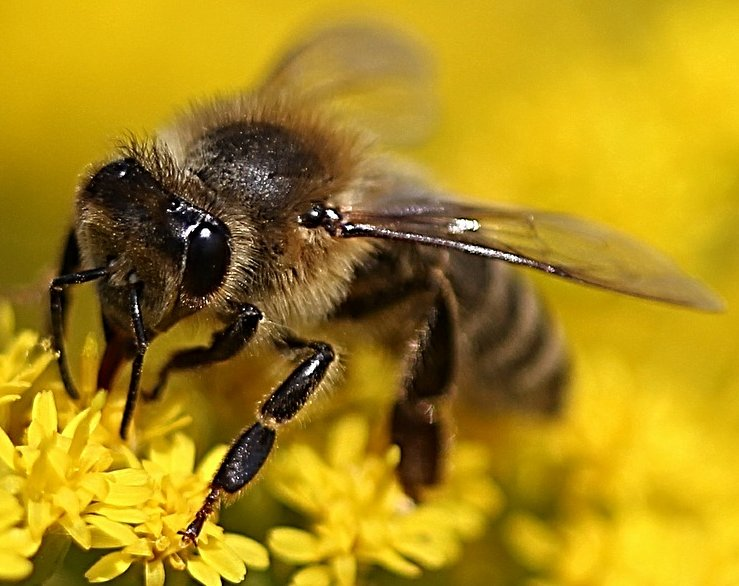
\includegraphics[width=\textwidth,keepaspectratio]{bee-593920_1920.jpg}
    \caption[Biene]{Apis Melferia - Frontalansicht einer Biene.}
    \label{fig:bee}
\end{figure}

Formeln im Text können mit Dollarzeichen dargestellt werden wie z. B. $x = 42$. Source code kann so wie in Listing \ref{lst:code} in Latex eingebaut werden, sollte jedoch nur wenige Zeilen haben.

\begin{lstlisting}[caption={Some example Code.}\label{lst:code},captionpos=b,language=Python] 
import numpy as np

def fun(x):
    return x + 1
\end{lstlisting}


\chapter{Resultate} % (fold)
\label{chap:resultate}

Tabellen, wie Tabelle \ref{tab:example} können auch mit einem Tabllengenerator wie auf Seite \url{https://www.tablesgenerator.com} im Internet erstellt werden.
\begin{table}[h]
    \centering
    \begin{tabular}{|r||l|l|}\hline
        t & $P(C_1)$ & $P(C_2)$\\\hline
        a & $0,6$ & $0,4$\\\hline
        b & $0,1$ & $0,9$\\\hline
        c & $0,82$ & $0,18$\\\hline\hline
        Mittelwert & \textbf{0,507} & $0,493$\\\hline
    \end{tabular}
    \caption{Beispiel für eine Tablle. Neben $Formeln$ und \textbf{Fettdruck} ist auch \textit{Kursiv} möglich.}
    \label{tab:example}
\end{table}


\chapter{Diskussion} % (fold)
\label{chap:diskussion}

Aufzählung sind auch sehr einfach:

\begin{enumerate}
    \item erster Punkt
    \item zweiter Punkt
    \begin{enumerate}
        \item erster Unterpunkt
        \item zweiter Unterpunkt
    \end{enumerate}
    \item weiter Punkt
\end{enumerate}

\blindtext


\chapter{Fazit und Ausblick} % (fold)
\label{chap:fazit}

Man kann auch \textbf{\textit{Fett und Kursiv}} kombinieren.

\begin{itemize}
    \item erster Punkt
    \item zweiter Punkt
    \begin{itemize}
        \item ein Unterpunkt
        \item noch ein Unterpunkt
    \end{itemize}
    \item ein weiterer Punkt
\end{itemize}

					% hier steht der eigentliche Text der Arbeit

\glsaddall[types={symbolslist}]

% \thispagestyle{empty}\null%\newpage

% \pagenumbering{Roman}

\listoffigures                          % Abbildungsverzeichnis
\listoftables                           % Tabellenverzeichnis

% \appendix
% \addchap{Anhang}
% \refstepcounter{chapter}
% % \pagestyle{plain}
% \fancyhead{Anhang}

\blindtext


% \lstlistoflistings
% \listofalgorithms

\setlength\bibitemsep{11pt}
\printbibliography              % Literaturverzeichnis

% \pagestyle{empty}

\end{document}
